\section{Results}
\label{sec:results}

\subsection{Score Fidelity}
\label{sec:results-score}

Figure~\ref{fig:main-mae} compares historical caching,
difficulty-stratified fixed subsets with weighted and gp-IRT estimation, and
Rasch adaptive testing on 287 held-out runs\footnote{Appendix report
complete values in tables.}.
We examine the remaining design choices within each method family in
Section~\ref{sec:results-design}.


\begin{figure}[t]
  \centering
  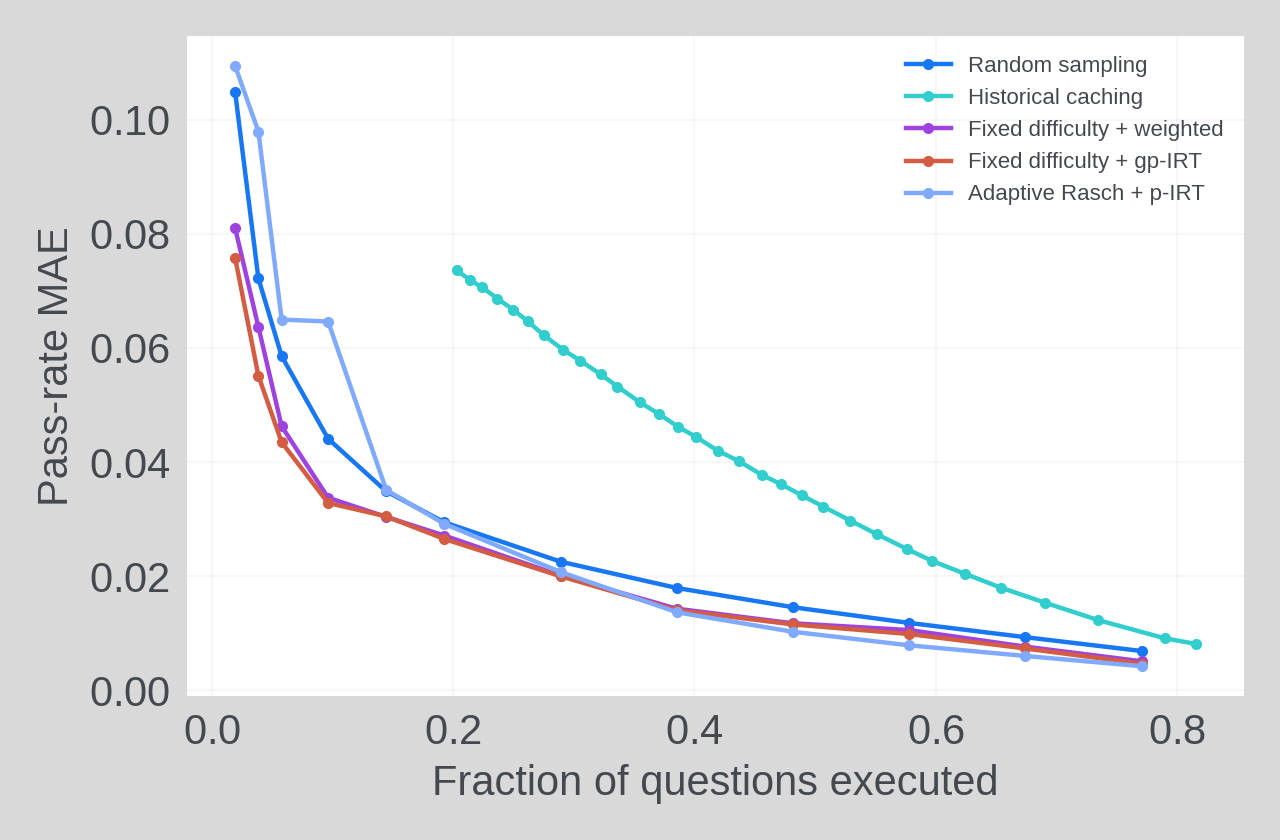
\includegraphics[width=0.9\columnwidth]{figures/main_mae_efficiency.png}
  \caption{Pass-rate MAE v.s. execution fraction.
     Fixed-budget methods use $k/519$. Caching points report mean execution
     fractions across cache thresholds.}
  \label{fig:main-mae}
  \vspace{-0.75em}
\end{figure}

Among the methods evaluated at fixed computational budgets $k$, difficulty-stratified subsets lead at small budgets: at $k{=}100$ (19.3\% of the benchmark), gp-IRT obtains
2.65pp MAE, compared with 2.94 for random sampling and 2.92
for adaptive testing. Adaptive testing leads from $k{=}200$ (38.5\%), where its MAE is 1.37
pp versus 1.40 for fixed-subset gp-IRT and 1.79 for random sampling. At $k{=}300$ (57.8\%),
the respective errors are 0.79, 0.99, and 1.18 pp. Weighted and gp-IRT subset
estimates are similar across these budgets.

Caching determines execution through its eligibility threshold, yielding mean
execution fractions from 20.3\% to 81.6\% and MAE from 7.36 to 0.81 pp. More
aggressive caching reduces execution but increases error, and its curve lies
above the other methods over their shared range. For example, caching obtains
1.54 pp MAE at 69.1\% execution, while adaptive testing, fixed-subset gp-IRT,
and random sampling obtain 0.60, 0.73, and 0.93 pp at $k{=}350$ (67.4\%).


\paragraph{Takeaway.}
Difficulty-stratified fixed subsets perform best at small budgets, while adaptive testing achieves the lowest MAE from $k{=}200$ onward. Historical caching is less accurate than the other methods at comparable execution levels.


\subsection{Ranking Fidelity}
\label{sec:results-ranking}

Fig.~\ref{fig:main-ranking} reports ranking fidelity for the same
configurations. Both correlations increase with the computational budget, but the differences among methods are more pronounced for Kendall's Tau.
At $k{=}100$ (19.3\%), fixed-subset gp-IRT obtains 0.930 Spearman and 0.770 Kendall,
compared with 0.923\&0.760 for adaptive testing and 0.911\&0.751 for random sampling. 
% The weighted estimation is similar to gp-IRT.

\begin{figure*}[t]
  \centering
  \begin{minipage}[t]{0.45\textwidth}
    \centering
    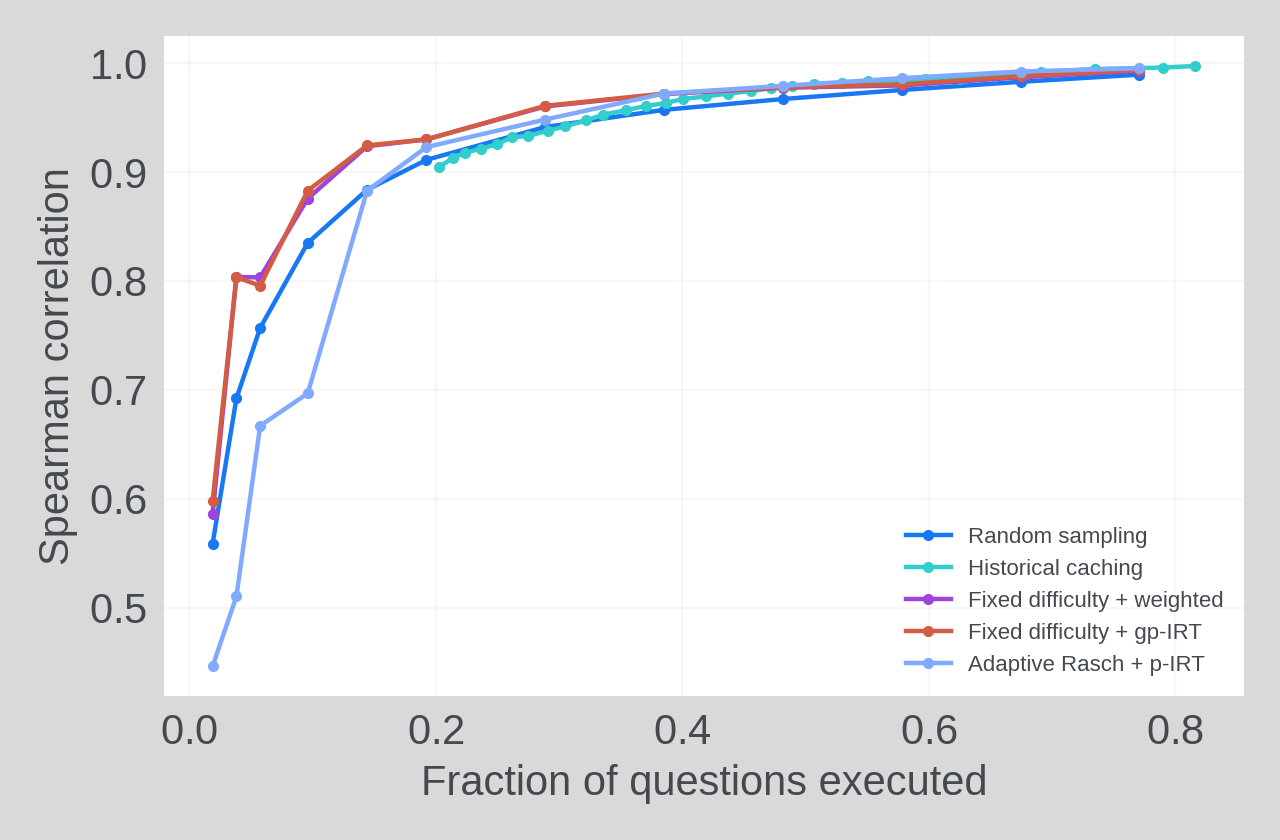
\includegraphics[width=\linewidth]{figures/main_spearman_efficiency.png}
    \small (a) Spearman correlation
  \end{minipage}\hfill
  \begin{minipage}[t]{0.45\textwidth}
    \centering
    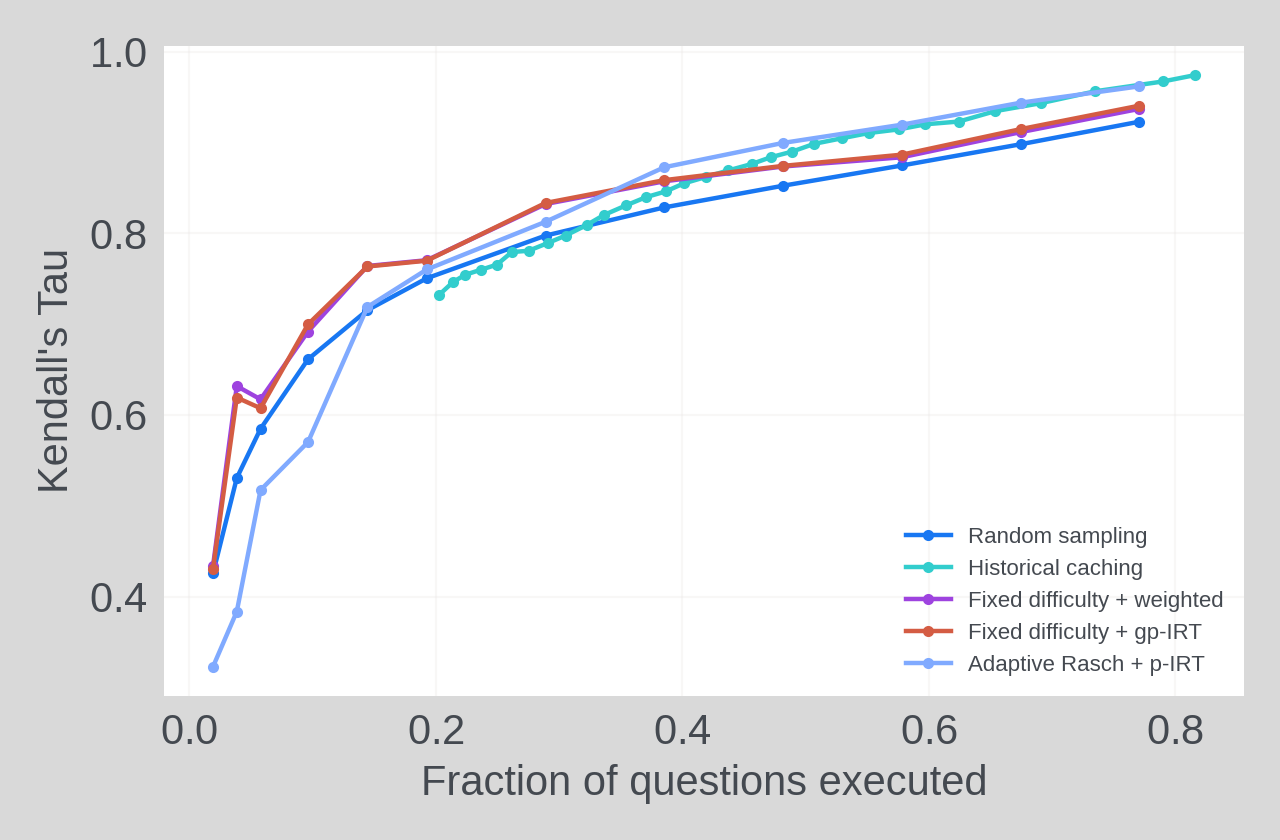
\includegraphics[width=\linewidth]{figures/main_kendall_efficiency.png}
    \small (b) Kendall's Tau
  \end{minipage}
  \vspace{-0.75em}
  \caption{Ranking fidelity v.s. execution fraction on 287 held-out runs.
  Higher is better.}
  \label{fig:main-ranking}
  \vspace{-0.75em}
\end{figure*}

Adaptive testing becomes stronger as the computational budget increases.
At $k{=}200$ (38.5\%), adaptive testing and fixed-subset gp-IRT tie in Spearman
(0.972), while adaptive testing has higher Kendall (0.873 v.s. 0.859). At
$k{=}300$ (57.8\%), adaptive testing reaches 0.986 Spearman and 0.920 Kendall,
compared with 0.981\&0.887 for fixed-subset gp-IRT and 0.975\&0.875 for
random sampling across budgets.

Caching preserves rankings much better than its score MAE suggests. At 20.3\%
execution it obtains 0.905 Spearman and 0.733 Kendall. At 79.0\%, it reaches
0.996 and 0.967, compared with 0.995 and 0.962 for adaptive testing at $k{=}400$
(77.1\%). 

\paragraph{Takeaway.}
Difficulty-stratified subsets give the strongest ranking fidelity at small
budgets, while adaptive testing leads at larger budgets. Historical caching
preserves run rankings substantially better than its score-estimation error
alone would suggest.

\subsection{Design Choices within Method Families}
\label{sec:results-design}

The score and ranking fidelity comparisons in
Sections~\ref{sec:results-score} and~\ref{sec:results-ranking} yield
similar method orderings. We therefore focus on MAE in
the remaining analyses and report rank
correlations in the appendix.

\subsubsection{Fixed-Subset Selection and Estimation}
Figure~\ref{fig:fixed-subset-mae} separates the effect of subset selection from
score estimation.
Difficulty stratification has the lowest MAE across most budgets and leads under
both estimators from $k{=}150$ (28.9\%). With gp-IRT, historical-response K-means
leads from $k{=}30$ (5.8\%) through $k{=}100$ (19.3\%) and generally outperforms
IRT-feature K-means. From $k{=}200$ (38.5\%), both clustering selectors perform
worse than random sampling under either estimator, while difficulty
stratification remains better.

\begin{figure}[t]
  \centering
  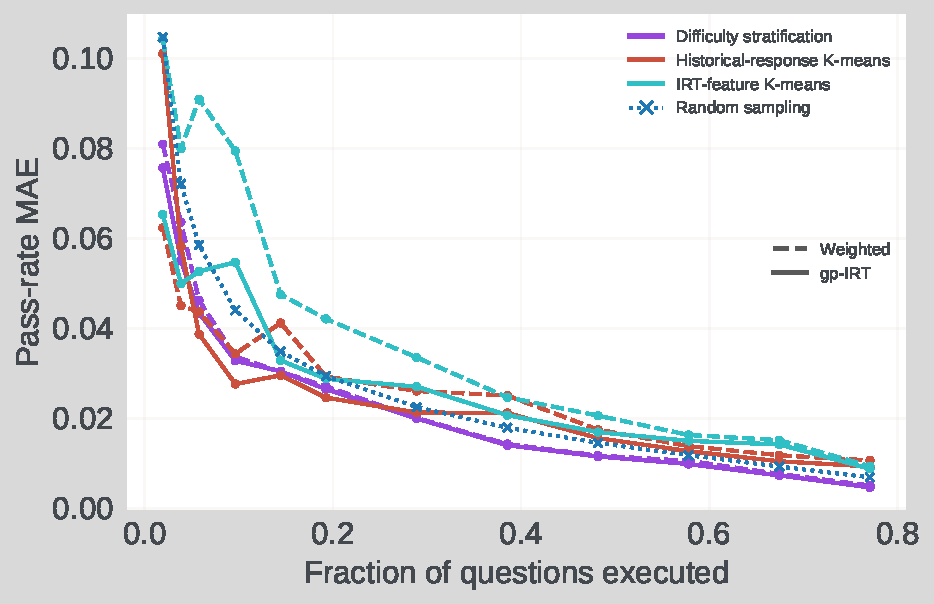
\includegraphics[width=0.9\columnwidth]{figures/fixed_subset_mae.pdf}
  \caption{Fixed-subset MAE on 287 held-out runs.}
  \label{fig:fixed-subset-mae}
  \vspace{-0.75em}
\end{figure}

gp-IRT benefits the clustering selectors more than difficulty stratification,
whose weighted and gp-IRT estimates are consistently similar. Ranking correlation results largely mirror MAE (Fig.~\ref{fig:fixed-subset-spearman}\&\ref{fig:fixed-subset-kendall}).

The weak performance of IRT-feature K-means contrasts with \citet{maiapolo2024tinybenchmarks}, which found IRT-based selection consistently effective. Two differences between the experimental settings may explain the conflicts.
First, our calibration data of recurring configurations of one production agent may contain fewer
distinct response patterns than diverse LLM populations used by \citet{maiapolo2024tinybenchmarks}, making multidimensional item parameters less reliable and therefore clusters less representative.
Difficulty stratification requires only a scalar difficulty ordering and directly preserves coverage across that range.
Second, our subsets are much larger fractions of the benchmark: $k{=}100$ (19.3\%) versus 100 of roughly 14,000 MMLU questions in \citet{maiapolo2024tinybenchmarks}. 
Random sampling becomes more accurate at these larger sampling fractions, leaving less scope for clustering to improve upon it.

\paragraph{Takeaway.}
Difficulty stratification performs best overall, while the more complex
selectors provide no consistent gain and fall below random sampling at moderate computational 
budgets.

\subsubsection{Adaptive IRT Model}

Figure~\ref{fig:adaptive-model-mae} compares Rasch and multidimensional 2PL
adaptive testing.
Multidimensional 2PL adaptive testing has lower MAE than Rasch and random
sampling at every $k$, with its largest advantage at $k{=}100$ (19.3\%):
1.97 pp versus 2.92 and 2.94 pp, respectively. Its advantage narrows as execution increases. Spearman and Kendall show the same ordering (Figure~\ref{fig:adaptive-model-ranking}).

\begin{figure}[t]
  \centering
  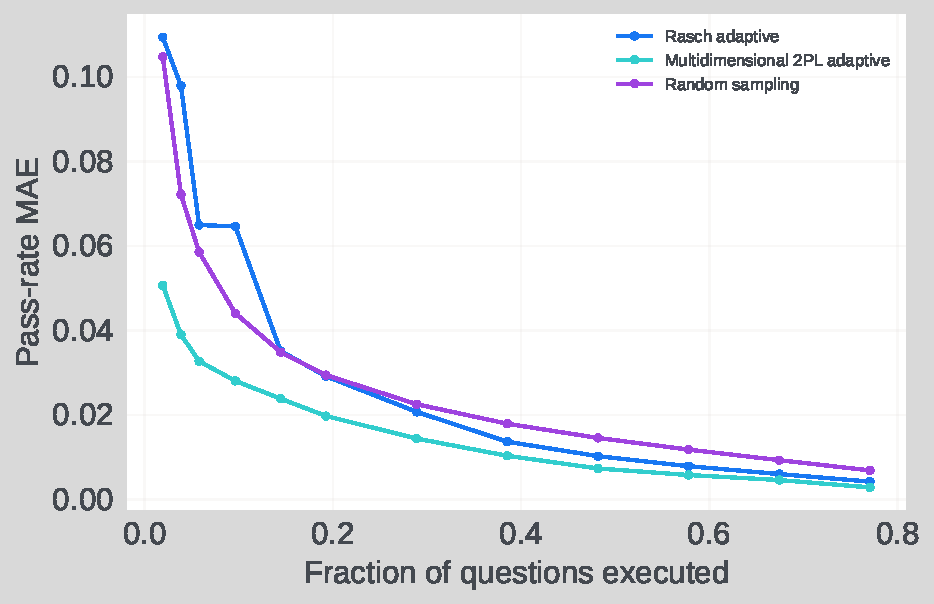
\includegraphics[width=0.9\columnwidth]{figures/adaptive_model_mae.pdf}
  \caption{Adaptive Testing MAE on the held-out runs.}
  \label{fig:adaptive-model-mae}
  \vspace{-0.75em}
\end{figure}

Rasch represents each run on one ability axis, whereas multidimensional 2PL
allows question outcomes to depend on different ability coordinates through
their discrimination vectors. D-optimal selection can therefore choose questions that inform ability coordinates not well covered by the questions already executed. This benefit is
largest at small computational budgets. As execution increases, p-IRT
replaces more predictions with observations, reducing the models' difference.

\paragraph{Takeaway.}
A more expressive IRT model can substantially improve adaptive testing.

\section{Practical Validation of Fixed-Subset}
\label{sec:fixed-validation}

The preceding comparisons show that difficulty-stratified fixed subsets provide
strong score and ranking fidelity. Although multidimensional adaptive testing
achieves lower error, difficulty stratification is operationally simpler: the
subset is constructed once and requires neither sequential selection nor
run-specific ability updates. Executing the same questions in every run also
supports direct question-level comparisons and diagnosis as the production
agent evolves. These properties motivated its use in our production workflow.

We therefore validate two properties important for recurring evaluation on difficulty-stratified fixed subset only:
whether a subset calibrated on one agent transfers to other agent families, and
how its fidelity changes with the calibration window.


\subsection{Cross-Agent Transfer}
\label{sec:cross-agent-transfer}

We apply the difficulty-stratified subsets and Rasch and gp-IRT parameters
calibrated on the original agent, without recalibration, to 299 runs from five
additional agent families. These distinct systems differ in their agent
frameworks, execution harnesses, tool sets, and model configurations. No
outcomes from these families are used to select questions or fit the estimators. We compare against uniform random sampling over the same computational budgets, averaged over 20 seeds.

On the pooled transferred runs, gp-IRT has lower MAE than random sampling at 11
of 12 budgets (Figure~\ref{fig:cross-agent-transfer}). At $k{=}200$ (38.5\%),
random sampling, weighted estimation, and gp-IRT obtain 1.86, 1.49, and 1.47 pp
MAE, respectively; gp-IRT also remains close to its 1.40 pp MAE on the original
287 held-out runs. Both fixed-subset estimators also exceed random sampling in
Spearman and Kendall correlation at every budget
(Figure~\ref{fig:cross-agent-transfer-ranking}).


\begin{figure}[t]
  \centering
  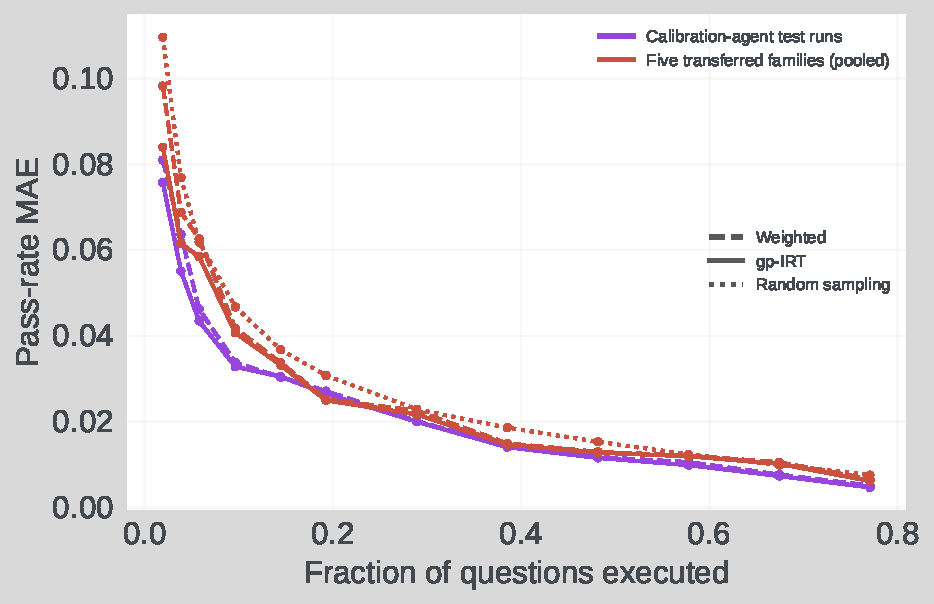
\includegraphics[width=0.9\columnwidth]{figures/cross_agent_transfer_mae.pdf}
  \caption{MAE on 287 original-agent and 299 transferred runs from five
  families. The subset and estimators use only original-agent calibration data.}
  \label{fig:cross-agent-transfer}
  \vspace{-0.75em}
\end{figure}
The advantage is not uniform across every family and computational budget. Nevertheless, gp-IRT has lower MAE than random sampling for a majority of budgets within each family. The appendix reports complete pooled and family-level results.


This transfer indicates that the IRT model captures intrinsic aspects of question difficulty that generalize across agent systems, even when calibrated on a single agent.

\paragraph{Takeaway.}
Without recalibration, the difficulty-stratified subset outperforms random
sampling on the pooled transferred runs at 11 of 12 budgets and remains close
to its original-agent fidelity, although gains vary across families.

\subsection{Calibration-Window Sensitivity}
\label{sec:calibration-window}

We next examine how the amount and time span of calibration data affect the
fixed subset. 
We fix the calibration end day at Day 28 and advance its start day in three-day increments from Day 1 to Day 28, 
yielding ten nested windows containing 287 to 14 runs (Table~\ref{tab:calibration-window-complete}).
For each window, we refit Rasch
and gp-IRT, reconstruct the difficulty-stratified subsets for
$k\in\{100,200,300,400\}$, and evaluate them on the same 287 held-out runs.

MAE does not increase monotonically as the calibration window shortens
(Fig.~\ref{fig:calibration-window-mae}). Variation is greatest at $k{=}100$. At $k{=}200$, gp-IRT MAE ranges from 1.35-1.59 pp: the
one-day window (14 runs) obtains 1.41 pp, compared with 1.40 pp for the full
four-week window. Weighted and gp-IRT estimates remain similar, while Spearman
and Kendall show the same non-monotonic pattern
(Fig.~\ref{fig:calibration-window-spearman}\&\ref{fig:calibration-window-kendall}).


\begin{figure}[t]
  \centering
  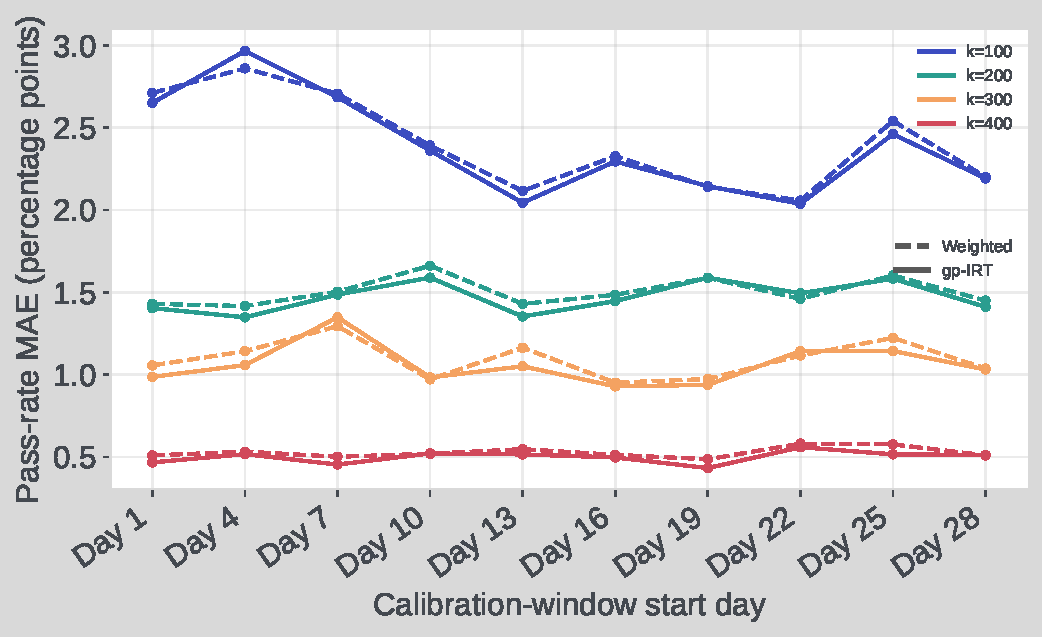
\includegraphics[width=0.9\columnwidth]{figures/calibration_window_mae.pdf}
  \caption{MAE across different calibration windows on 287 held-out runs.}
  \label{fig:calibration-window-mae}
  \vspace{-0.75em}
\end{figure}

This stability may reflect the relatively mature development stage of the agent
and limited day-to-day change during the study. Recent runs may therefore
suffice to estimate the difficulty ordering used for stratification and may
better match the immediately following test period, while older runs add limited new information.

\paragraph{Takeaway.}
Fixed-subset fidelity is stable across the studied calibration windows,
with no consistent benefit from retaining the full 4-week history.
